
\documentclass[11pt]{article}
%\Large
\usepackage{epsf}
%\usepackage{fontinst}
\usepackage{amsmath}
\usepackage{amssymb}
\bibliographystyle{alpha}
%\usepackage{helvetic}
\usepackage{fancybox}
\usepackage{fancyvrb}
\usepackage{shadow}
\usepackage{verbatim}
\usepackage{lscape}
\usepackage[dvips]{graphicx}
\usepackage{float}
%\usepackage{style/fancyheadings}
\usepackage{makeidx}
%\usepackage{psfig}
%\usepackage{style/doublespace}
\usepackage{pstricks,pst-node,pst-tree}

%\usepackage{times}
\usepackage{palatino}
%\include{my_environ}
%for version counter



% environment for computer listing

\renewcommand{\thefootnote}{\fnsymbol{footnote}}

\begin{document}
\author{ Andi Klein \\ pabloemma@gmail.com}
\title{ test\_speed program1\_3 LCWA \\ 
		\bf{version: 1.0}}
%\date{12 Nov 2002}
%\today
\maketitle
% set the counter level depth
\setcounter{secnumdepth}{10}
\setcounter{tocdepth}{10}

\tableofcontents

\newenvironment{andilist}{\begin{itemize} \em}{\end{itemize}}



\section{Overview}
test\_speed is a python program written by Andi Klein. It's main purpose is to collect data from different raspberry pi's distributed across the LCWA to check the bandwidth over 24 hours. This is strictly a program for \textbf{La Canada Wireless Association}, which is a notforprofit volunteer organization , which provides internet access to mostly rural communities around Santa Fe.If you want to use this code for other places, feel free to modify it to suit your needs.

The heart of the code are calls to the \textbf{Ookla} speedtest servers and/or the \textbf{iperf3} library. 

The test gets executed every 10 minutes and the data are stored locally. Every hour the program connects to dropbox, and uploads the datafile and the plot file. At midnight every day, the program flushes all the data to dropbox and exits. The computer then does a git pull to a central repository, performs a pull and the restarts. This ensures that any program updates are caught by the clients.
Until 2022, the program was using Ookla's speedtest and reporting those numbers. As is documented below, the user can choose the Ookla server, according to their preferences. Over time it has become clear that we would like to have a speedtest which is strictly within the LCWA network, and not a combination of this network and the internet. Several times we noticed strange test resulst, which were driven by an overloaded Ookla server and not a degradation of the LCWA network. This led to the development of a new addition to the code using iperf3. This iperf3 connection goes to a LCWA iperf3 server, therefore providing a more honest picture of what is going on in our network. This program runs on \textbf{Mac} and \textbf{Linux} but \textbf{NOT} on Windows. There are currently no plans to ever port it to Windows.

\section{Installation and upgrade}

Before you can do anything, you have to clone the repo. Create a directory ~/git/speedtest with mkdir -p ~git/speedtest.

\begin{itemize}
\item cd git/speedtest
\item git clone https://github.com/pabloemma/LCWA .
\item if you need a different branch: git fetch; git branch -v -a; git checkout branchname
%\item cd ../src
%item ./install\_speedtest  2$>$\&1 $|$ tee install.log

\end{itemize}
The program has many components, which rely on different python and system packages. I hope I have them all in the install script. If you run in difficulties, send me the output of the installation.

Sometimes I will make changes which require an upgrade, and then the script upgrade\_speedtest will be run.

\vspace{3cm}

\subsection{Installing on a Linux raspberry pi system}
In this case you should be able to use the provided install script : install|\_speedtest. There is also a mac installation script, but this is currently outdated.
\begin{verbatim}

 cd ../src
 ./install_speedtest  2>&1 | tee install.log
\end{verbatim}

If the installation crashes, please send me the install.log file.

\subsection{general instructions for running the system on your own}
In the following a discussion on what you need to install the project:
\begin{enumerate}
\item	Install the speedtest CLI from  https://www.speedtest.net/apps/cli
\item Once installed you need to run it once to accept the license
\item pip install dropbox
%\item pip install pycryptodome
\item Mac: brew install git, Linux it is usually supplied, otherwise sudo apt get install git , or yum install git
\item mkdir ~/speedfiles (below your home directory)
\item mkdir git
\item cd git
\item git clone https://github.com/pabloemma/speedtest.git speedtest (this you only do once, after this your command will be git pull , which will update you to the latest version)
\item You will need a dropbox account and setup an app. If you have a dropbox account, log in and then go to https://www.dropbox.com/developers/documentation, click on ``App console'' in the upper right corner and create a new app. There click on permission type and select which one you want. Once you generated the app, click on the button Generate under``Generated Access Token ''
\item Copy into clipboard the Access token, which is very long
\item open the file LCWA\_d.txt in your speedtest directory, remove the line and paste your access token.
\item On dropbox also create a folder called ``LCWA'', this is where the files will go.
\end{enumerate}


\begin{enumerate}
\item install iperf3 \textbf{(not iperf or iperf2)}
\end{enumerate}



\section{Running and controlling the program}

The program has currently two different ways to run; either speedtest, which is a wrapper around the OOkla speedtest  or iperf, which will run an iperf test to a server on the LCWA network. The issue with the Ookla server is, that the result is depending on quite a few parameters beyond LCWA's control. The current server is with cybermesa,
and we have noticed that the server is sometimes slow. Also, since we go outside onto the internet, the results are  influenced by whatever traffic is going on. The iperf test really checks thge available bandwidth within the LCWA network, and is therefore a better measure of what we provide.

The program checks every 10 minutes the bandwith, and records this is a file in the directory /home/pi/speedfiles. Every hour around xx:30 the csv file gets plotted into a pdf file and both are shipped to the corresponding dropbox.
At midnight a second program collates all the different speedboxes, and creates a full 24 plot file. Also at midnight the program terminates, performs a git pull for updates, and then restarts again. In order not to blast the servers at the same time, each speedbox has a delay in the startup corresponding to the 2 digits in the name.
\begin{equation}
delay = XX*25
\end{equation}
where the XX stands for the two digit speedboxnumber (LC04) would mean 04  as the multiplier and leads to a 100 sec delay.

\subsection{Required directory settings}

In order for me to support the program, I require the following directory structure:

/home/pi/git/speedtest is where all the components for the speedtest are located. The data files produced will be in /home/pi/speedfiles . If you choose a different configuration, you have to change the config file and you are on your own.
 

\subsection{config file}
Here is an example of a config file:
\begin{verbatim}
{

    "Darwin" : {
        "timeout" : "/usr/local/bin/timeout",
        "speedtest" : "/usr/local/bin/speedtest",
        "srcdir" : "/Users/klein/visual studio/LCWA/src/",
        "datadir" : "/Users/klein/speedfiles/",
        "conf_dir" : "/Users/klein/visual studio/LCWA/config/"

    },
    "Linux" : {
        "timeout" : "/usr/bin/timeout",
        "speedtest" : "/usr/bin/speedtest",
        "srcdir" : "/home/pi/git/speedtest/src/",
        "datadir" : "/home/git/speedfiles/",
        "conf_dir" : "/home/pi/git/speedtest/src/config/"

    },
    "Control" : {
        "runmode" : "Iperf",
        "debug"   : false,
        "cryptofile" : "LCWA_d.txt"
    },
    "Iperf" : {
        "serverport"  : "5201",
        "serverip" : "63.229.162.245",
        "duration"  : 10,
        "numstreams" : 2,
        "blksize"   : 1024,
        "latency_ip" : "65.19.14.51",
        "time_window" : 10,

        "reverse"   : false
    },
    "Speedtest" : {
        "serverip" : "63.229.162.245",
        "serverid" : 18002,
        "time_window" : 10,
        "latency_ip" : "65.19.14.51" 
    }
        "ClusterControl" : {
        "LC01" :  {
            "runmode" : "Both",

            "nondefault" : {

                    "server_ip" :"63.229.162.245" ,
                    "serverid" : 18002,
                    "time_window" : 10,
                    "latency_ip" : "65.19.14.51" ,
                    "iperf_serverport"  : "5201",
                    "iperf_serverip" : "63.229.162.245",
                    "iperf_duration"  : 30,
                    "iperf_numstreams" : 2,
                    "iperf_blksize"   : 1024,
                    "iperf_latency_ip" : "65.19.14.51",
                    "iperf_time_window" : 10,
            
                    "iperf_reverse"   : false,
                    "random" : true
                     }

                    },

}

\end{verbatim}

As you can see , this is a json file (which personally I don't like; who in their right mind develops a system, which does not allow comments) and we can look at it in some more details:

The first two block deal with the runtime environment. Since Apple and Linux have their stuff not in the same location (thank you apple) , we have to specify the locations of some critical files and directories. The next block \textbf{Control} deal;s with issues which are common to both runmodes and operating systems. \textbf{Iperf} selects the iperf test, while \textbf{Speedtest} controls space aliens (just kidding and making sure you haven't fallen asleep yet).

The last two blocks contain control parameters used for the two different runmodes.

If you choose Both for the running, you should also provide the variable random in the control block and set it to either true or false. If false, the program will switch back and forth between iperf and speedtest on a regular basis, indeed every time it should run . If you set random to true, it will decide randomly which way to go.

I added a clustercontrol block, where you can fine tune the parameters for every speedbox. If you don't change anything in the clustercontrol, it takes the default values.

\subsection{Running}

Everything is controlled through two crontab entries, one on the user level and one the sudo level.
The root level one starts the system after the midnight exit, and the user one restarts the program if for some reaso it exits. Here are the two crontab settings:

The first one you get with sudo crontab -e
\begin{verbatim}
 Edit this file to introduce tasks to be run by cron.
# 
# Each task to run has to be defined through a single line
# indicating with different fields when the task will be run
# and what command to run for the task
# 
# To define the time you can provide concrete values for
# minute (m), hour (h), day of month (dom), month (mon),
# and day of week (dow) or use '*' in these fields (for 'any').
# 
# Notice that tasks will be started based on the cron's system
# daemon's notion of time and timezones.
# 
# Output of the crontab jobs (including errors) is sent through
# email to the user the crontab file belongs to (unless redirected).
# 
# For example, you can run a backup of all your user accounts
# at 5 a.m every week with:
# 0 5 * * 1 tar -zcf /var/backups/home.tgz /home/
# 
# For more information see the manual pages of crontab(5) and cron(8)
# 
# m h  dom mon dow   command
@reboot sleep 60 ;  /home/pi/git/speedtest/scripts/run_speedtest >>/home/pi/run_speedtest.log
\end{verbatim}

The second one is just crontab -e and looks like this:
\begin{verbatim}
.....
.....
# For more information see the manual pages of crontab(5) and cron(8)
# 
# m h  dom mon dow   command
*/10 * * * * /home/pi/git/speedtest/scripts/restart.sh

# run every hour at 55 minues
55 * * * * /home/pi/git/speedtest/scripts/git_pull.sh

59� 23 * * * /home/pi/git/speedtest/scripts/git_pull.sh

\end{verbatim}

where I only show the last few lines

% end of definitions

\section{Results}

Below is the typical output of one of the speedboxes for a 24 hr period. During this time, Lumen had huge problems with delivering our bandwidth and this is reflected in the black squares, which measure the download speed to a speedtest server. The red triangles are the uploadspeed to the same server. In contrast the blue and green are our iperf results, which test the bandwidth within our network.


\begin{figure}[H]%                 use [hb] only if necceccary!
  \centering
  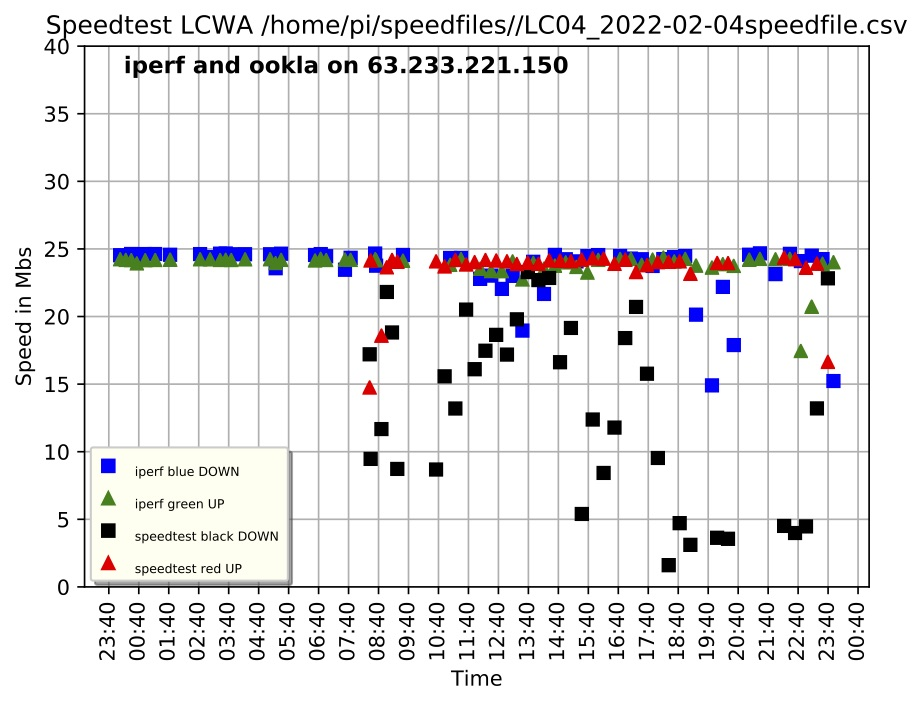
\includegraphics[width=8cm]{LC04_2022-02-04speedfile.jpg}
  \caption{LC04 on Feb 04 2022}
  \label{fig:LC04}
\end{figure}

There are three files produced with extensions pdf, csv and txt. The csv file contains the raw data , the pdf is a plot of the data and the txt file has a list of parameters the program run under, plus at midnight a statistics output.
In the following the midnight output from the plotted run. The important info are the run conditions at the beginning, which in this case is \textbf{Both} , and then the different parameters for iperf and speedtest.

\begin{verbatim}
IP    63.233.221.150
Date    2022-02-04 23:50:47.244401
Dropbox    /LCWA/LC04_/
MacAddress    b8:27:eb:41:62:97
File    LC04_2022-02-04speedfile.csv
version    8.02.01
runmode    Both
iperf server    63.229.162.245
iperf port    5201
iperf numstreams    2
iperf blocksize    1024
iperf duration    30
iperf reverse    False
time window    600
ookla server id    18002
latency ip    65.19.14.51
random    False


 ********************************total statistics********************** 
Iperf 
Min download                 = 14.903761103996434
Max download                 = 24.66901502375453
Mean download                 = 23.558043052947266
Std download                 = 2.128372106266123
Min upload                 = 17.440534244451296
Max upload                 = 24.34935391081165
Mean upload                 = 23.83621240450195
Std upload                 = 1.015410482611458


Ookla Speedtest 
Min download                 = 1.598744
Max download                 = 23.282152
Mean download                 = 13.355808000000001
Std download                 = 6.769985371569937
Min upload                 = 14.74664
Max upload                 = 24.351616
Mean upload                 = 23.40635557894737
Std upload                 = 2.067538460635904


 ********************************end statistics********************** 


\end{verbatim}


\end{document}
